\chapter{Marco  Teórico}

En el presente capítulo se explican conceptos y terminología relacionada al diseño inverso de dispositivos fotónicos.
Para ello se desarrolla tres secciones. 
En primer lugar, se describe las propiedades físicas de interés de un \emph{bend} y WDM.
En segundo lugar, se desarrolla en cinco pasos como utilizar el diseño inverso para optimizar los dispositivos de estudio.
  \begin{itemize}
  \item Se especifica tres estrategias comúnmente usadas para parametrizar la región de diseño.
  \item Se muestra como definir la función objetivo para un \emph{bend} y WDM.
  \item Se señala los programas donde se puede simular el comportamiento de los diseños que desarrollemos.
  \item Se expone como se explican estrategias de optimización para un dispositivo fotónico.
  \item Se da a conocer transformaciones que se pueden incluir al plan de optimización para incorporar restricciones de fabricación.
  \end{itemize}  
En tercer lugar, se explica la conversión de los resultados de la optimización a un formato listo para ser fabricado.


\section{Dispositivos de estudio}

\subsection{\emph{Bend}}

Un \emph{bend} es un dispositivo fotónico que se encarga de guiar un haz de ondas para que gire.

En general, al estudiar dispositivos fotónicos es de especial interés la distribución del campo eléctrico. 
Este campo se descompone en una componente transversal eléctrica (TE) y en una componente transversal magnética (TM) de acuerdo a la siguiente ecuación:

\begin{equation}
  E = E^{TE} + E^{TM}
\label{eq:field}
\end{equation}

Donde $E^{TE}$ es la componente paralela al dispositivo y $E^{TM}$ es la componente restante \citep{Hohenester2020}. 

La intensidad de estos campos es de especial interés pues nos dan una idea del rendimiento del dispositivo. 
Por ejemplo, en la figura \ref{fig:efield} se muestra la intensidad del campo $E^{TE}$ cuando un haz de luz está pasándo por el dispositivo. 
Como podemos observar, parte del campo está fuera del \emph{bend} representado por color azul oscuro.
Así, se visualiza de forma gráfica que el dispositivo está teniendo considerables pérdidas de energía lo cual es un indicador de un mal rendimiento.


\begin{figure}[ht]
  \centering
  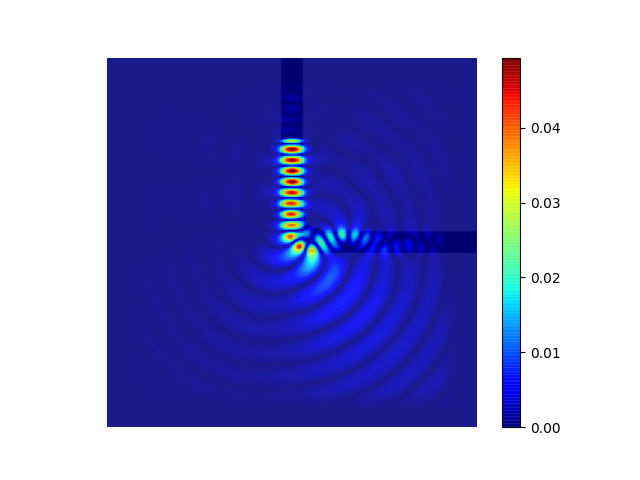
\includegraphics[scale=0.8]{image/theory/bend-field.png}
  \caption{Intensidad de campo eléctrico para un \emph{bend-90°} de radio interno de 0.25 $\mu m$}
  \label{fig:efield}
\end{figure}

Por otro lado, para evaluar el desempeño de un \emph{bend} de forma numérica se suele calcular la transmitancia como la relación entre la intensidad del haz que sale del dispositivo con la intensidad con la que entra. Esto se expresa mediante la ecuación \ref{eq:transmission}:

\begin{equation}
  T = \frac{I}{I_0}
\label{eq:transmission}
\end{equation}

Ahora, por temas de implementación, es común calcular lo que se conoce como \emph{overlap} ya que es un buen indicador de tener una buena transmitancia \citep{Su2020}.

\subsection{\emph{Wavelength Demultiplexer} de dos canales (WDM)}

Un WDM es un dispositivo fotónico que se encarga de guiar un haz de ondas de acuerdo a su longitud de onda.
Así, estos suelen trabajar con dos longitudes de onda y guían las de un tipo por la guía de onda superior y las de otro tipo por la guía de onda inferior.

Similar al caso del \emph{bend} se estudia su campo eléctrico y su transmitancia para medir el rendimiento de estos dispositivos.

\section{Diseño inverso}

\subsection{Parametrización}

Tres estrategias comúnes para parametrizar un dispositivo fotónico son: i) parametrización por píxeles, ii) parametrización por conjuntos de nivel, iii) parametrización por segmentos.

\subsubsection{Parametrización basada en topología}

A cada píxel se le asocia un valor dado por la fórmula \ref{eq:permitivity} \citep{Su2020}:

\begin{equation}
  \varepsilon(x, y) = \varepsilon_{Si} + (1 - \lambda_{x,y}) \varepsilon_{SiO_2} \quad \lambda_{x, y} \in [0, 1], \lambda_{x, y} \in \mathbb{R} 
\label{eq:permitivity}
\end{equation}

Donde $\varepsilon_{Si} = 3.48$ es la permitividad del $Si$ y $\varepsilon_{SiO_2} = 1.44$ es la permitividad del $SiO2$.
Con esta ecuación se mapea el intervalo $[0, 1]$ con el intervalo $[1.44, 3.48]$. 
Esto se realiza para determinar la permitividad que hay en la ubicación del píxel y poder simular las ecuaciones de Maxwell en el dispositivo.
Con esta parametrización obtenemos una cantidad infinita de diseños, mas solo nos interesan aquellos donde $\lambda_{x,y}$ es entero, pues en caso contrario un píxel se mapea a la permitividad de un material desconocido lo cual lo volvería infabricable.


En la figura \ref{fig:pixeles} se muestra la parametrización por píxeles de un \emph{bend-90°}. 
Las píxeles en gris representan regiones donde se está usando una permitividad desconocida, es decir se ha tomado un $\lambda_{x,y}$ no entero.

\begin{figure}[h]
  \centering
  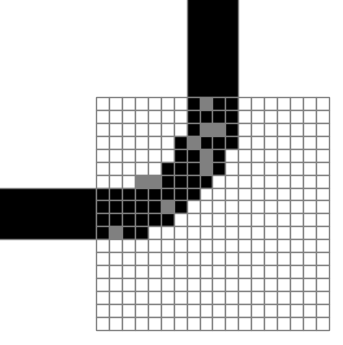
\includegraphics[scale=0.8]{image/theory/parametrization-pixeles.png}
  \caption{Parametrización por píxeles para un \emph{bend-90°}}
  \label{fig:pixeles}
\end{figure}


\subsubsection{Parametrización por conjuntos de nivel}

A cada píxel se le asocia una permitividad dada por la siguiente fórmula \citep{Piggott2017}:

  \[ \varepsilon(x, y) =
    \begin{cases}
      \varepsilon_{Si}       & \quad \text{si } \phi(x, y) \leq 0\\
      \varepsilon_{SiO_2}    & \quad \text{si } \phi(x, y) > 0
    \end{cases}
  \]

Donde $\phi$ se define como una función contínua. 
En la figura \ref{fig:levelsets} se muestra como esta parametrización permite mantener curvas continuas para representar al dispositivo (líneas amarillas).
Luego, los píxeles intentan cubrir la región definida por estas curvas para después poder simular numéricamente las propiedades del dispositivo.

\begin{figure}[h]
  \centering
  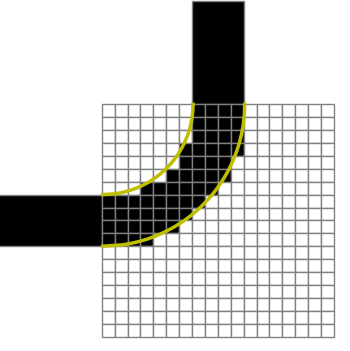
\includegraphics[scale=0.8]{image/theory/parametrization-levelsets.png}
  \caption{Parametrización por conjuntos de nivel para un \emph{bend-90°}}
  \label{fig:levelsets}
\end{figure}




\subsubsection{Parametrización por segmentos}

Con esta estrategia se considera la región de diseño como un rectángulo y se lo divide en $n$ segmentos de igual tamaño. 
Luego, el tamaño de cada segmento será un parámetro y la geometría se forma a partir de estos valores considerando ubicar cada segmento centrado verticalmente. 
En la figura \ref{fig:splines} podemos observar como \cite{Prosopio-Galarza2019} utiliza esta parametrización con $13$ segmentos para diseñar un 2-splitter.


\begin{figure}[ht]
  \centering
  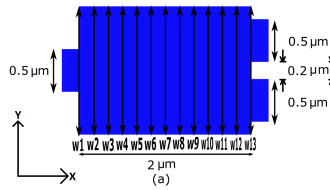
\includegraphics[scale=0.8]{image/theory/parametrization-spline.png}
  \caption{Parametrización por 13 segmentos de un \emph{2-splitter}. Imagen extraída de \cite{Prosopio-Galarza2019}}
  \label{fig:splines}
\end{figure}


Las distintas estrategias de parametrización mostradas tienen sus propias características.
La parametrización por segmentos asegura simetría y regiones compactas, pero tiene un espacio de búsqueda más reducido que las otras opciones.
Por otro lado, la parametrización por píxeles trabaja con un espacio de búsqueda mucho más grande a cambio de poder parametrizar diseños no fabricables.
En cambio, la parametrización por niveles se encarga de mantener una función continua con el fin de mantener el diseño similar a como terminará el dispositivo fabricado.

\subsection{Definición de la función objetivo}

La función objetivo es un valor asociado a una parametrización que nos permite comparar distintas parametrizaciones para determinar que diseño es mejor. 
En el área de fotónica es común referirse a esta función como la figura de mérito (FOM). 
Basándonos en \cite{Su2020} se tiene que conviene definir la FOM de la siguiente manera:

\begin{enumerate}

\item \emph{Bend}

\begin{equation}
  f_{obj}(p) = max \left \{ T(p) \right \}
\label{eq:fom-bend}
\end{equation}

Es decir, la función objetivo asociada a la parametrización $p$ es maximizar la transmitancia, ver equación \ref{eq:transmission}, asociada a esa parametrización.

\item WDM

La función objetivo se define como:

\begin{equation}
  f_{obj}(p) = max \left \{ g_0(p, 0)^2 + (1 - g_0(p, 1))^2 + g_1(p, 1)^2 + (1 - g_1(p, 0))^2 \right \}
\label{eq:fom-splitter}
\end{equation}

Donde $g_0(p, i)$ representa la transmitancia asociada a la parametrización $p$ en la guía de onda $i$ para una longitud de onda de $1400 nm$ y 
      $g_1(p, i)$ representa su análogo para una longitud de onda de $1550 nm$.

La ecuación \ref{eq:fom-splitter} busca maximizar la transmitancia por la guía de onda superior y minimizarla para la guía de onda inferior cuando se recibe una longitud de onda de $1400 nm$ y lo contrario para una longitud de onda de $1550 nm$.

\end{enumerate}

\subsection{Simulación}

Existen distintas librerías de Python que nos permiten definir dispositivos fotónicos en base a lo descrito. 
Dos librerías muy usadas para ello son MEEP \citep{Oskooi2010} y SPINS \citep{Su2020}. 
Una evaluación cualitativa de sus funcionalidades puede ser vista en la tabla \ref{tab:simulation}.

\begin{table}[ht]
    \centering
    \begin{tabular}{|c|c|c|c|c|}
    \hline 
    Librería &  Usabilidad & Eficiencia & Bugs & Funcionalidad \\
    \hline 
    MEEP &  Difícil & Alta & Elevados & Extensa \\
    SPIN &  Moderada  & Moderada-Alta & Pocos & Básica necesaria \\
    \hline 
    \end{tabular}
    \caption{Evaluación cualitativa de las librerías MEEP y SPINS}
    \label{tab:simulation}
\end{table}


\subsection{Estrategias de optimización}

La forma de optimizar un diseño depende de la parametrización utilizada. De esta forma, tenemos los siguientes casos:

\begin{enumerate}


\item{Parametrización por píxeles}


La ecuación \ref{eq:permitivity} ya señala un rango de valores asociados a cada píxel. 
Pero, para asegurar el obtener un diseño fabricable se divide la optimización en dos pasos \citep{Su2020}:

  \begin{enumerate}
  \item Optimización continua
  
  Se varía el valor de $\lambda_{x,y}$ en el intervalo $[0, 1]$ sin importar si se obtiene diseños no fabricables.

  \item Optimización discreta

  Se considera el resultado de la optimización continua como punto inicial del algoritmo de optimización.
  Luego, se va aplicando una transformación que permita ir convergencia a una parametrización donde cada $\lambda_{x, y}$ tenga un valor entero.
  Algunos ejemplos de estas transformaciones se pueden encontrar en la siguiente sección.

  \end{enumerate}

\item{Parametrización por conjuntos de nivel}

Como lo detalla \cite{Piggott2017}, con este tipo de parametrización es conveniente utilizar una optimización basada en la gradiente y
asegurar convergencia con una búsqueda en línea.

\item{Parametrización por segmentos}

Basándonos en \cite{Prosopio-Galarza2019}, con este tipo de parametrización conviene definir un rango de posibles valores para cada segmento.
Luego, ejecutar algún algoritmo de optimización, de preferencia uno de optimización global, para finalmente tratar de incorporar restricciones de fabricación en una etapa posterior.

\end{enumerate}

\subsection{Transformaciones}

La aplicación de transformaciones a un diseño se realiza con el fin de obtener dispositivos con curvas suaves para asegurar un buen desempeño al momento de fabricarse \citep{Su2020}. 
De acuerdo al tipo de parametrización utilizada, tenemos:

\begin{itemize}
  \item Para el caso de la parametrización por segmentos, si queremos suavizar el diseño obtenido podemos considerar las alturas de los segmentos e interpolar una curva \citep{Yangjin2013}.

  \item Para el caso de la parametrización por conjunto de nivel se define $\phi$ de forma que asegure curvas suaves, así no es necesario aplicar transformaciones.

  \item Para el caso de la parametrización por píxeles, una forma se suavizar las regiones punteagudas es aplicar una función de suavizado conforme va iterando el algoritmo de optimización aplicado. Basándonos en \cite{Zhang2021}, podemos aplicar la siguiente función:

\begin{equation}
  s(p) = \frac{\tanh (\beta \times \eta) + \tanh (\beta \times (p - \eta))}{\tanh (\beta \times \eta) + \tanh (\beta \times (1 - \eta))}
  \label{eq:topo-smooth}
\end{equation}

    Donde $p$ es la parametrización del dispositivo, $\eta = 0.5$ y $\beta$ comienza con un valor de 1 y va incrementándose exponencialmente en cada iteración. 
    Como se observa en la figura \ref{fig:discretization}, la ecuación \ref{eq:topo-smooth} se encarga de ir haciendo converger los valores de la parametrización a $0$ o $1$ de acuerdo a cual esté más cercano. 
    Conforme aumenta el valor de $\beta$ esta convergencia es más rápida.

    \begin{figure}[ht]
      \centering
      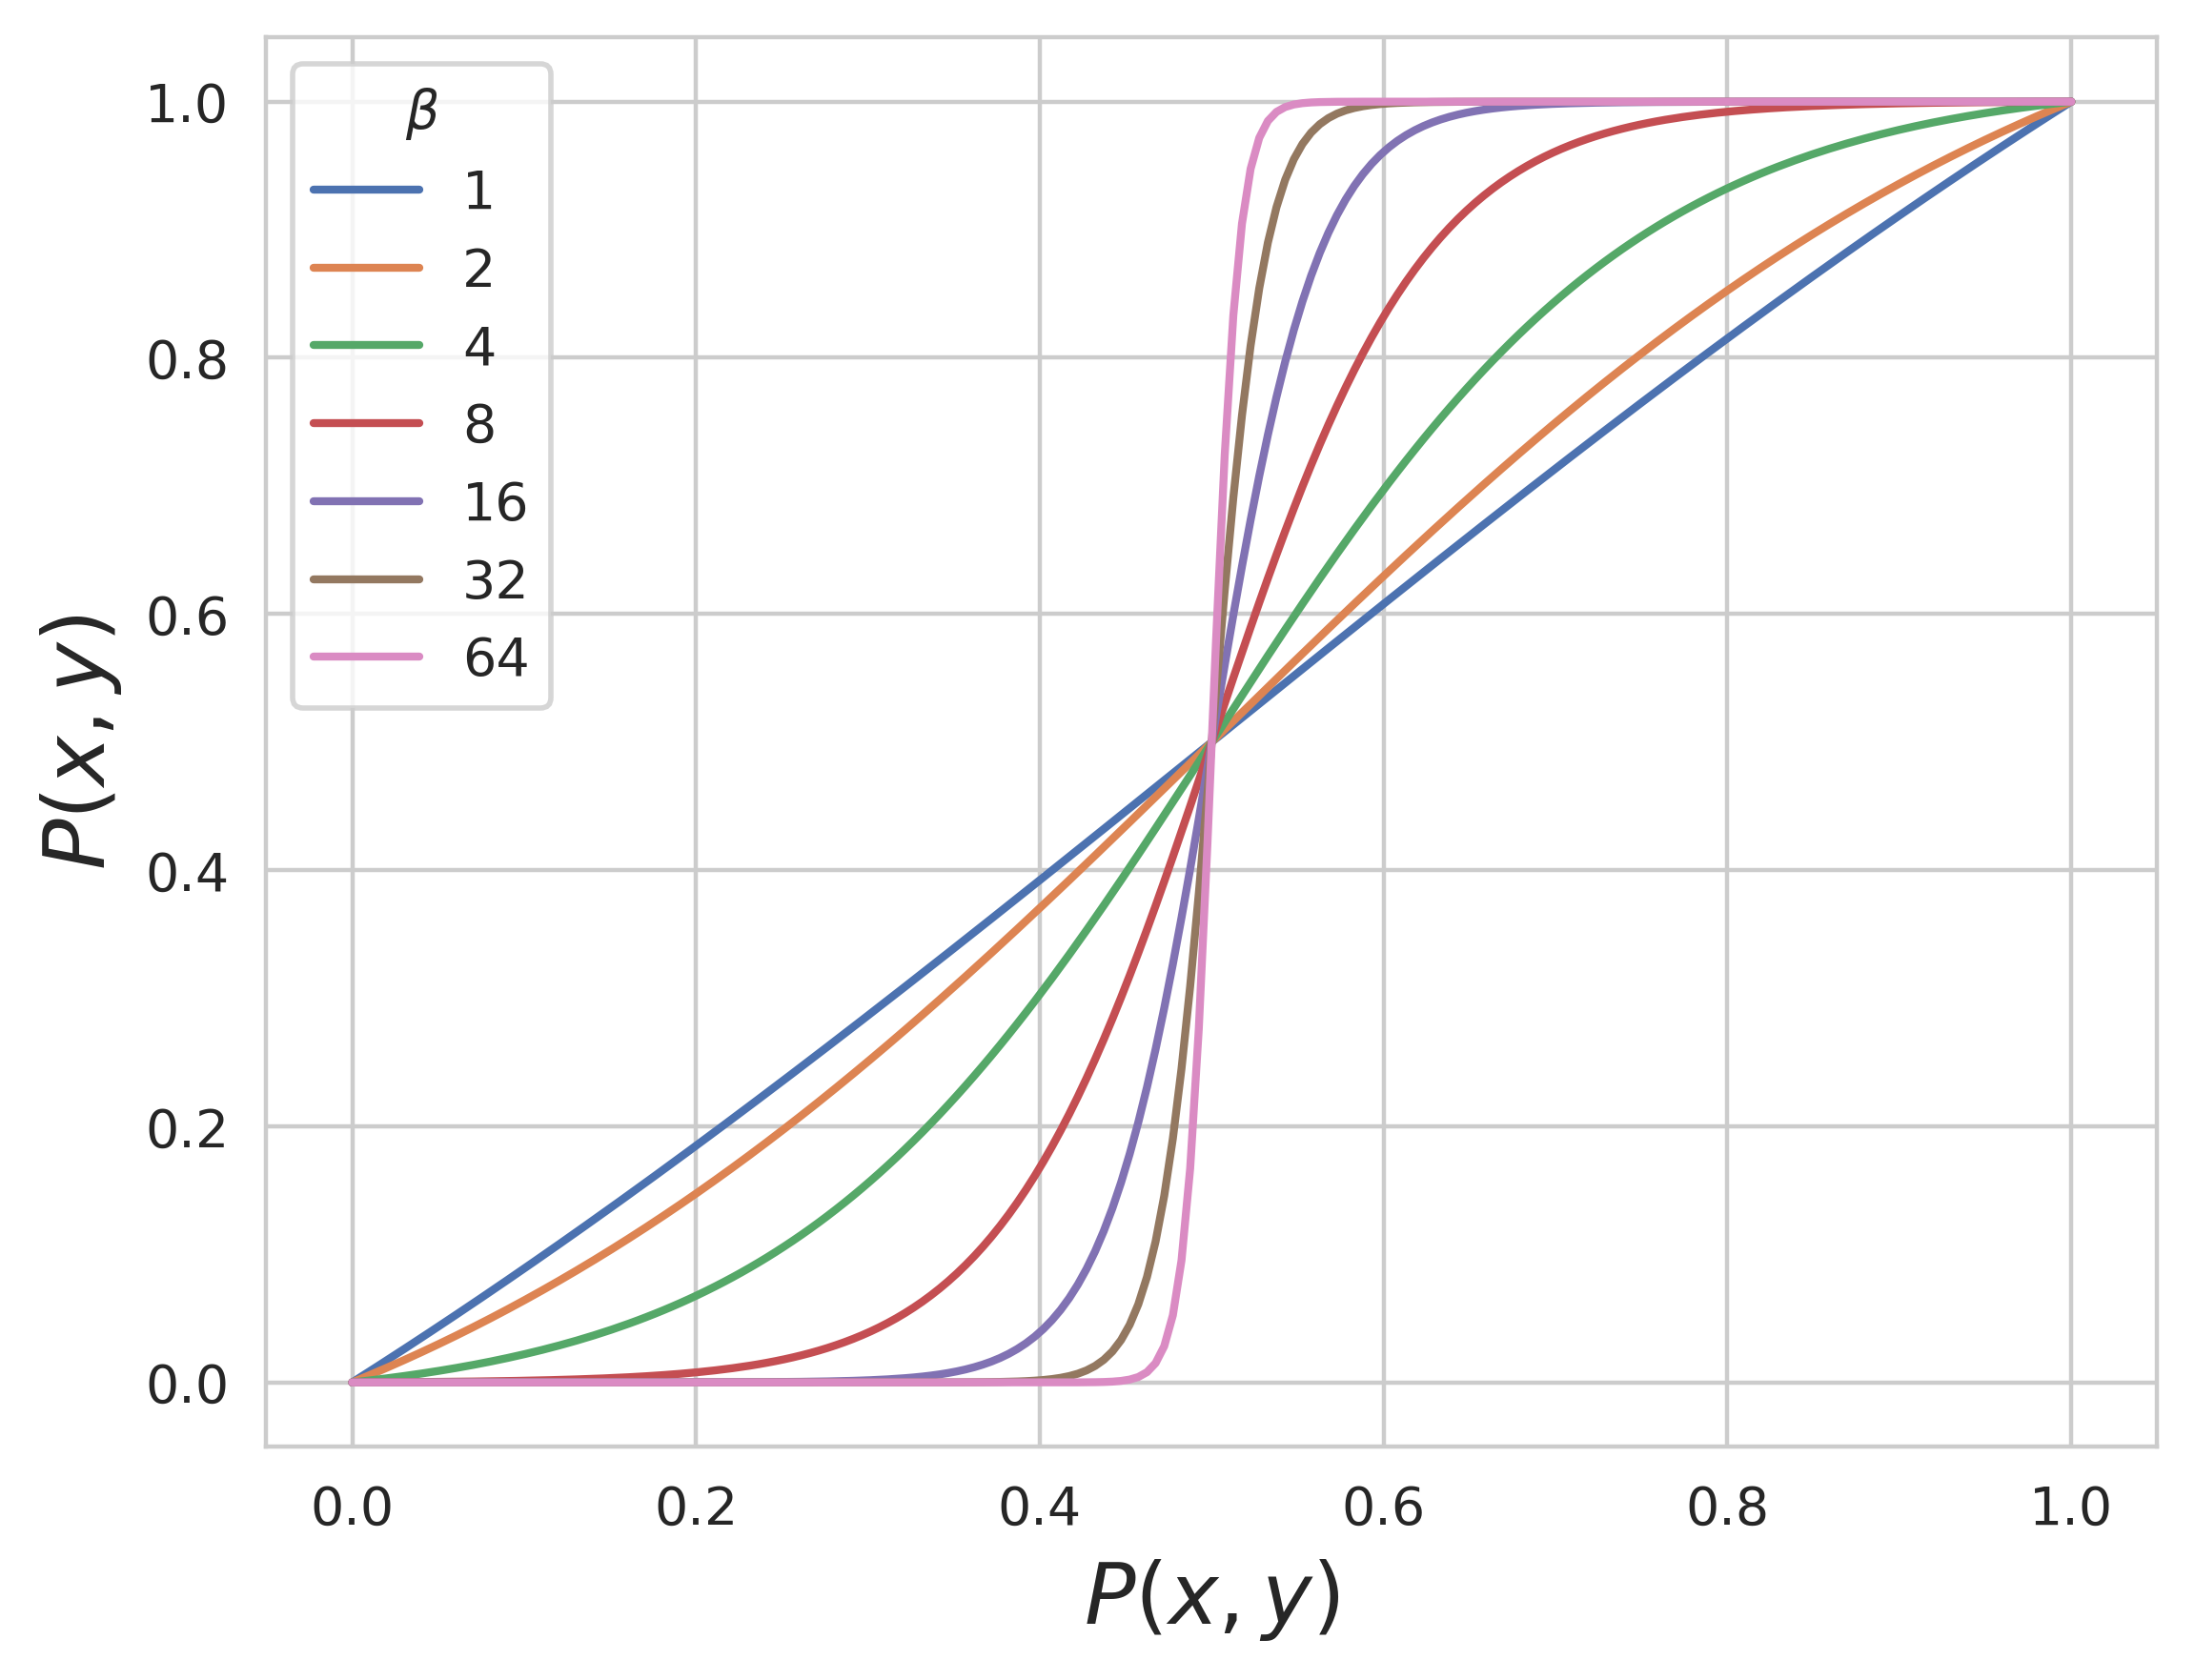
\includegraphics[scale=0.8]{image/theory/discretization.png}
      \caption{Función de discretización con $eta = 0.5$ y distintos valores de $\beta$}
      \label{fig:discretization}
    \end{figure}

\end{itemize}

